\documentclass[12pt,letterpaper]{article}
\usepackage{graphicx,textcomp}
\usepackage{natbib}
\usepackage{setspace}
\usepackage{fullpage}
\usepackage{color}
\usepackage[reqno]{amsmath}
\usepackage{amsthm}
\usepackage{fancyvrb}
\usepackage{amssymb,enumerate}
\usepackage[all]{xy}
\usepackage{endnotes}
\usepackage{lscape}
\newtheorem{com}{Comment}
\usepackage{float}
\usepackage{hyperref}
\newtheorem{lem} {Lemma}
\newtheorem{prop}{Proposition}
\newtheorem{thm}{Theorem}
\newtheorem{defn}{Definition}
\newtheorem{cor}{Corollary}
\newtheorem{obs}{Observation}
\usepackage[compact]{titlesec}
\usepackage{dcolumn}
\usepackage{tikz}
\usetikzlibrary{arrows}
\usepackage{multirow}
\usepackage{xcolor}
\newcolumntype{.}{D{.}{.}{-1}}
\newcolumntype{d}[1]{D{.}{.}{#1}}
\definecolor{light-gray}{gray}{0.65}
\usepackage{url}
\usepackage{listings}
\usepackage{color}

\definecolor{codegreen}{rgb}{0,0.6,0}
\definecolor{codegray}{rgb}{0.5,0.5,0.5}
\definecolor{codepurple}{rgb}{0.58,0,0.82}
\definecolor{backcolour}{rgb}{0.95,0.95,0.92}

\lstdefinestyle{mystyle}{
	backgroundcolor=\color{backcolour},   
	commentstyle=\color{codegreen},
	keywordstyle=\color{magenta},
	numberstyle=\tiny\color{codegray},
	stringstyle=\color{codepurple},
	basicstyle=\footnotesize,
	breakatwhitespace=false,         
	breaklines=true,                 
	captionpos=b,                    
	keepspaces=true,                 
	numbers=left,                    
	numbersep=5pt,                  
	showspaces=false,                
	showstringspaces=false,
	showtabs=false,                  
	tabsize=2
}
\lstset{style=mystyle,
 basicstyle=\linespread{0.9}\ttfamily\small,
columns=flexible,
keepspaces=true,
aboveskip=4pt,
belowskip=4pt
}
\newcommand{\Sref}[1]{Section~\ref{#1}}
\newtheorem{hyp}{Hypothesis}

\title{Problem Set 3}
\date{Due: November 12, 2026}
\author{Applied Stats/Quant Methods 1}


\begin{document}
	\maketitle
	\section*{Instructions}
	\begin{itemize}
		\item Please show your work! You may lose points by simply writing in the answer. If the problem requires you to execute commands in \texttt{R}, please include the code you used to get your answers. Please also include the \texttt{.R} file that contains your code. If you are not sure if work needs to be shown for a particular problem, please ask.
	\item Your homework should be submitted electronically on GitHub.
	\item This problem set is due before 23:59 on Thursday November 12, 2026. No late assignments will be accepted.

	\end{itemize}

		\vspace{.25cm}
	
\noindent In this problem set, you will run several regressions and create an add variable plot (see the lecture slides) in \texttt{R} using the \texttt{incumbents\_subset.csv} dataset. Include all of your code.

\newpage
\section*{Question 1}
\noindent We are interested in knowing how the difference in campaign spending between incumbent and challenger affects the incumbent's vote share. 
	\begin{enumerate}
		\item Run a regression where the outcome variable is \texttt{voteshare} and the explanatory variable is \texttt{difflog}. \\
		\begin{doublespace}
			\lstinputlisting[language=R, firstline=33, lastline=39]{PS03_answersJX.R}
		\begin{footnotesize}
			\begin{verbatim}
Call:
lm(formula = voteshare ~ difflog, data = inc.sub)

Residuals:
Min       1Q   Median       3Q      Max 
-0.26832 -0.05345 -0.00377  0.04780  0.32749 

Coefficients:
Estimate Std. Error t value Pr(>|t|)    
(Intercept) 0.579031   0.002251  257.19   <2e-16 ***
difflog     0.041666   0.000968   43.04   <2e-16 ***
---
Signif. codes:  0 ‘***’ 0.001 ‘**’ 0.01 ‘*’ 0.05 ‘.’ 0.1 ‘ ’ 1

Residual standard error: 0.07867 on 3191 degrees of freedom
Multiple R-squared:  0.3673,	Adjusted R-squared:  0.3671 
F-statistic:  1853 on 1 and 3191 DF,  p-value: < 2.2e-16
			\end{verbatim}
		\end{footnotesize}
		\end{doublespace}
		\item Make a scatterplot of the two variables and add the regression line. \\
		\begin{doublespace}
			\lstinputlisting[language=R, firstline=41, lastline=47]{PS03_answersJX.R}
			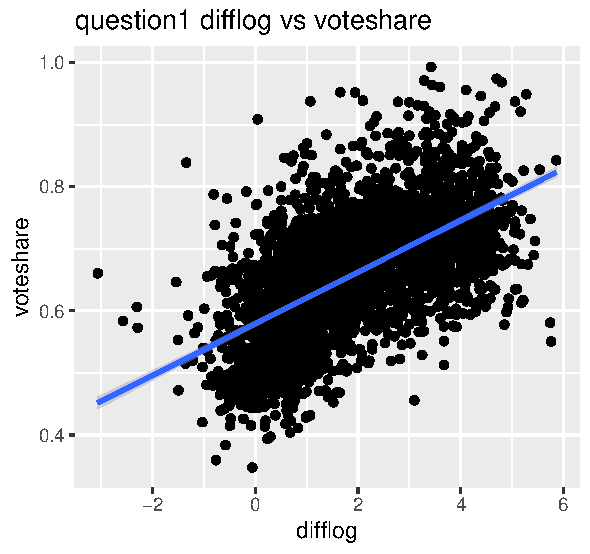
\includegraphics[width=.65\textwidth]{scattor_question1.pdf}
		\end{doublespace}
		
		\newpage
		\item Save the residuals of the model in a separate object.	\\
		\begin{doublespace}
			\lstinputlisting[language=R, firstline=49, lastline=50]{PS03_answersJX.R}
		\end{doublespace}
		\item Write the prediction equation.\\
		\begin{doublespace}
		\begin{footnotesize}
	\begin{verbatim}
		Coefficients:
		Estimate Std. Error t value Pr(>|t|)    
		(Intercept) 0.579031   0.002251  257.19   <2e-16 ***
		difflog     0.041666   0.000968   43.04   <2e-16 ***
	\end{verbatim}
	\end{footnotesize}
	From the summary of the regression model, we can find that the intercept is 0.579 and the slope is 0.042. We can write the prediction equation as:
	$$\hat{y} = 0.042x + 0.579$$
	where $y$ is \texttt{voteshare} and $x$ is \texttt{difflog}. On average, a one-unit increase in \texttt{difflog} is associated with a 0.042 unit increase in \texttt{voteshare}. This coefficient is statistically significant at the $\alpha = 0.05$ level ($p < 0.001$). When \texttt{difflog} is 0, the predicted \texttt{voteshare} is 0.579 (about 57.9\%).
		\end{doublespace}
	\end{enumerate}
	
\newpage

\section*{Question 2}
\noindent We are interested in knowing how the difference between incumbent and challenger's spending and the vote share of the presidential candidate of the incumbent's party are related.	\vspace{.25cm}
	\begin{enumerate}
		\item Run a regression where the outcome variable is \texttt{presvote} and the explanatory variable is \texttt{difflog}.	 \\
		\begin{doublespace}
			\lstinputlisting[language=R, firstline=58, lastline=60]{PS03_answersJX.R}
		\begin{footnotesize}
			\begin{verbatim}
Call:
lm(formula = presvote ~ difflog, data = inc.sub)

Residuals:
Min       1Q   Median       3Q      Max 
-0.32196 -0.07407 -0.00102  0.07151  0.42743 

Coefficients:
Estimate Std. Error t value Pr(>|t|)    
(Intercept) 0.507583   0.003161  160.60   <2e-16 ***
difflog     0.023837   0.001359   17.54   <2e-16 ***
---
Signif. codes:  0 ‘***’ 0.001 ‘**’ 0.01 ‘*’ 0.05 ‘.’ 0.1 ‘ ’ 1

Residual standard error: 0.1104 on 3191 degrees of freedom
Multiple R-squared:  0.08795,	Adjusted R-squared:  0.08767 
F-statistic: 307.7 on 1 and 3191 DF,  p-value: < 2.2e-16
			\end{verbatim}
		\end{footnotesize}
		\end{doublespace}
		\item Make a scatterplot of the two variables and add the regression line. 	 \\
		\begin{doublespace}
			\lstinputlisting[language=R, firstline=63, lastline=68]{PS03_answersJX.R}
			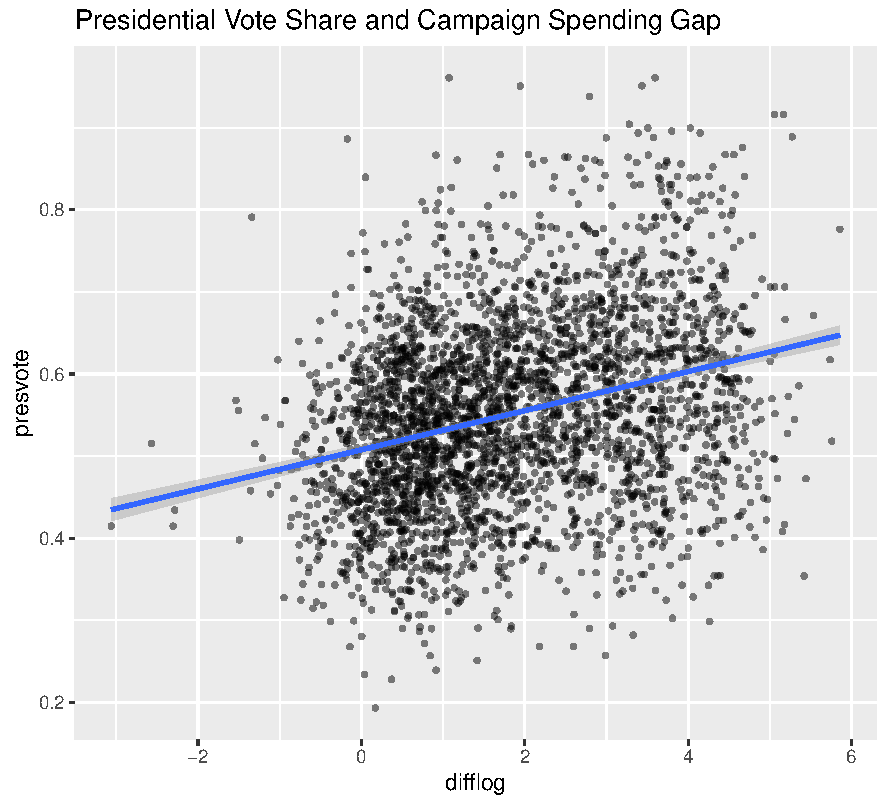
\includegraphics[width=.65\textwidth]{scattor_question2.pdf}
		\end{doublespace}
		
		\newpage
		\item Save the residuals of the model in a separate object.
		\begin{doublespace}
			\lstinputlisting[language=R, firstline=71, lastline=71]{PS03_answersJX.R}
		\end{doublespace}
		
		\item Write the prediction equation.\\
			\begin{doublespace}
			\begin{footnotesize}
			\begin{verbatim}
Coefficients:
Estimate Std. Error t value Pr(>|t|)    
(Intercept) 0.507583   0.003161  160.60   <2e-16 ***
difflog     0.023837   0.001359   17.54   <2e-16 ***
				\end{verbatim}
			\end{footnotesize}
			From the summary of the regression model, we can find that the intercept is 0.508 and the slope is 0.024. We can write the prediction equation as:
			$$\hat{y} = 0.024x + 0.508$$
			where $y$ is \texttt{presvote} and $x$ is the \texttt{difflog}. On average, one unit change in \texttt{difflog} is associated with 0.024 unit increase in \texttt{presvote}. This coefficient is statistically significant at the $\alpha = 0.05$ level ($p < 0.001$). When \texttt{difflog} is 0, the predicted \texttt{presvote} is 0.508 (about 50.8\%).
		\end{doublespace}
	\end{enumerate}
	
	\newpage	
\section*{Question 3}

\noindent We are interested in knowing how the vote share of the presidential candidate of the incumbent's party is associated with the incumbent's electoral success.
	\vspace{.25cm}
	\begin{enumerate}
		\item Run a regression where the outcome variable is \texttt{voteshare} and the explanatory variable is \texttt{presvote}.
		\begin{doublespace}
		\lstinputlisting[language=R, firstline=78, lastline=80]{PS03_answersJX.R}
		\begin{footnotesize}
			\begin{verbatim}
Call:
lm(formula = voteshare ~ presvote, data = inc.sub)

Residuals:
Min       1Q   Median       3Q      Max 
-0.27330 -0.05888  0.00394  0.06148  0.41365 

Coefficients:
Estimate Std. Error t value Pr(>|t|)    
(Intercept) 0.441330   0.007599   58.08   <2e-16 ***
presvote    0.388018   0.013493   28.76   <2e-16 ***
---
Signif. codes:  0 ‘***’ 0.001 ‘**’ 0.01 ‘*’ 0.05 ‘.’ 0.1 ‘ ’ 1

Residual standard error: 0.08815 on 3191 degrees of freedom
Multiple R-squared:  0.2058,	Adjusted R-squared:  0.2056 
F-statistic:   827 on 1 and 3191 DF,  p-value: < 2.2e-16
			\end{verbatim}
		\end{footnotesize}
	\end{doublespace}
		
		\newpage
		\item Make a scatterplot of the two variables and add the regression line. 
		\begin{doublespace}
		\lstinputlisting[language=R, firstline=83, lastline=88]{PS03_answersJX.R}
		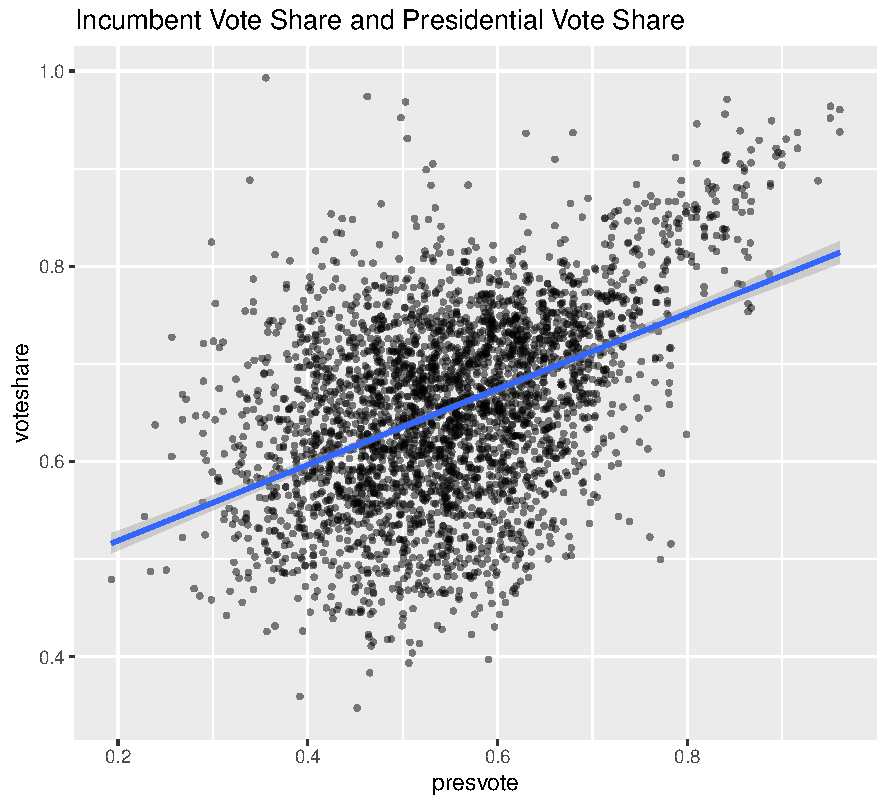
\includegraphics[width=.65\textwidth]{scattor_question3.pdf}
		\end{doublespace}
		
		\newpage
		\item Write the prediction equation.
		\begin{doublespace}
		\begin{footnotesize}
		\begin{verbatim}
Coefficients:
Estimate Std. Error t value Pr(>|t|)    
(Intercept) 0.441330   0.007599   58.08   <2e-16 ***
presvote    0.388018   0.013493   28.76   <2e-16 ***
		\end{verbatim}
		\end{footnotesize}
		From the summary of the regression model, we can find that the intercept is 0.441 and the slope is 0.388. We can write the prediction equation as:
			$$\hat{y} = 0.388x + 0.441$$
			where $y$ is \texttt{voteshare} and $x$ is the \texttt{presvote}. On average, one unit change in \texttt{presvote} is associated with 0.388 unit increase in \texttt{voteshare}. This coefficient is statistically significant at the $\alpha = 0.05$ level ($p < 0.001$). When \texttt{presvote} is 0, the predicted \texttt{voteshare} is 0.441 (about 44.1\%).
\end{doublespace}
	\end{enumerate}
	

\newpage	
\section*{Question 4}
\noindent The residuals from part (a) tell us how much of the variation in \texttt{voteshare} is $not$ explained by the difference in spending between incumbent and challenger. The residuals in part (b) tell us how much of the variation in \texttt{presvote} is $not$ explained by the difference in spending between incumbent and challenger in the district.
	\begin{enumerate}
		\item Run a regression where the outcome variable is the residuals from Question 1 and the explanatory variable is the residuals from Question 2.	\\
		\begin{doublespace}
			\lstinputlisting[language=R, firstline=94, lastline=96]{PS03_answersJX.R}
		\end{doublespace}
		
		\begin{footnotesize}
			\begin{verbatim}
				Call:
				lm(formula = res_question1 ~ res_question2)
				
				Residuals:
				Min       1Q   Median       3Q      Max 
				-0.25928 -0.04737 -0.00121  0.04618  0.33126 
				
				Coefficients:
				Estimate Std. Error t value Pr(>|t|)    
				(Intercept)   -5.934e-18  1.299e-03    0.00        1    
				res_question2  2.569e-01  1.176e-02   21.84   <2e-16 ***
				---
				Signif. codes:  0 ‘***’ 0.001 ‘**’ 0.01 ‘*’ 0.05 ‘.’ 0.1 ‘ ’ 1
				
				Residual standard error: 0.07338 on 3191 degrees of freedom
				Multiple R-squared:   0.13,	Adjusted R-squared:  0.1298 
				F-statistic:   477 on 1 and 3191 DF,  p-value: < 2.2e-16
			\end{verbatim}
		\end{footnotesize}
		\newpage
		\item Make a scatterplot of the two residuals and add the regression line. 	\\
		\begin{doublespace}
			\lstinputlisting[language=R, firstline=98, lastline=104]{PS03_answersJX.R}
			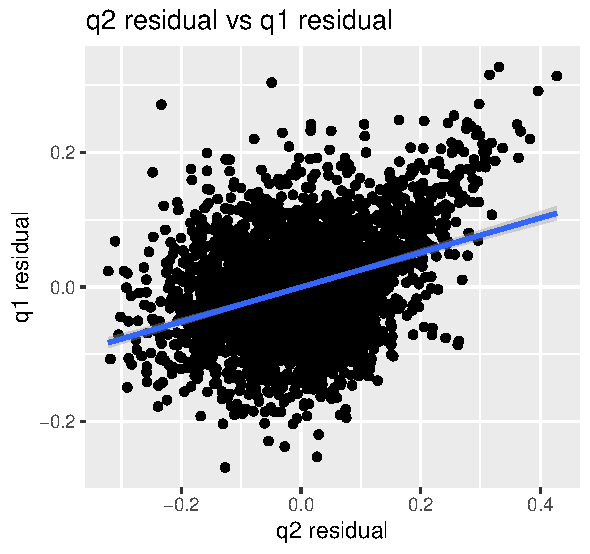
\includegraphics[width=.65\textwidth]{scattor_question4.pdf}
		\end{doublespace}
		\newpage
		\item Write the prediction equation.
		\begin{doublespace}
		\begin{footnotesize}
		\begin{verbatim}
Coefficients:
Estimate Std. Error t value Pr(>|t|)    
(Intercept)   -5.934e-18  1.299e-03    0.00        1    
res_question2  2.569e-01  1.176e-02   21.84   <2e-16 ***
		\end{verbatim}
		\end{footnotesize}
  		From the summary of the regression model, we can find that the intercept is $-5.934 \times 10^{-18}$, which is effectively 0, and the slope is 0.2569. We can write the prediction equation as:
		$$\hat{y} = 0.2569x$$
		where $y$ is the residuals from Question 1 and $x$ is the residuals from Question 2. The residuals from Question 1 are the part of \texttt{voteshare} not explained by \texttt{difflog}, and the residuals from Question 2 are the part of \texttt{presvote} not explained by \texttt{difflog}. On average, a one-unit increase in the Question 2 residuals is associated with a 0.257 increase in the Question 1 residuals.
\end{doublespace}
	\end{enumerate}
	
	\newpage	

\section*{Question 5}
\noindent What if the incumbent's vote share is affected by both the president's popularity and the difference in spending between incumbent and challenger? 
	\begin{enumerate}
		\item Run a regression where the outcome variable is the incumbent's \texttt{voteshare} and the explanatory variables are \texttt{difflog} and \texttt{presvote}.	
		\begin{doublespace}
		\lstinputlisting[language=R, firstline=107, lastline=109]{PS03_answersJX.R}
		\end{doublespace}
		\begin{footnotesize}
	\begin{verbatim}
Call:
lm(formula = voteshare ~ difflog + presvote, data = inc.sub)

Residuals:
Min       1Q   Median       3Q      Max 
-0.25928 -0.04737 -0.00121  0.04618  0.33126 

Coefficients:
Estimate Std. Error t value Pr(>|t|)    
(Intercept) 0.4486442  0.0063297   70.88   <2e-16 ***
difflog     0.0355431  0.0009455   37.59   <2e-16 ***
presvote    0.2568770  0.0117637   21.84   <2e-16 ***
---
Signif. codes:  0 ‘***’ 0.001 ‘**’ 0.01 ‘*’ 0.05 ‘.’ 0.1 ‘ ’ 1

Residual standard error: 0.07339 on 3190 degrees of freedom
Multiple R-squared:  0.4496,	Adjusted R-squared:  0.4493 
F-statistic:  1303 on 2 and 3190 DF,  p-value: < 2.2e-16
	\end{verbatim}
\end{footnotesize}
		\newpage
		\item Write the prediction equation.
		\begin{doublespace}
		\begin{footnotesize}
		\begin{verbatim}
			Coefficients:
			Estimate Std. Error t value Pr(>|t|)    
			(Intercept) 0.4486442  0.0063297   70.88   <2e-16 ***
			difflog     0.0355431  0.0009455   37.59   <2e-16 ***
			presvote    0.2568770  0.0117637   21.84   <2e-16 ***
		\end{verbatim}
		\end{footnotesize}
	From the summary of the regression model, we can find that the intercept is 0.449, the coefficient for \texttt{difflog} is 0.036, and the coefficient for \texttt{presvote} is 0.257. We can write the prediction equation as:
	$$\hat{y} = 0.449 + 0.036x_1 + 0.257x_2$$
	where $y$ is the incumbent's \texttt{voteshare}, $x_1$ is \texttt{difflog} and $x_2$ is \texttt{presvote}. On average, a one-unit increase in \texttt{difflog} is associated with a 0.036 unit increase in \texttt{voteshare}, holding \texttt{presvote} constant. On average, a one-unit increase in \texttt{presvote} is associated with a 0.257 unit increase in \texttt{voteshare}, holding \texttt{difflog} constant. Both coefficients are statistically significant at the $\alpha = 0.05$ level ($p < 0.001$). When both \texttt{difflog} and \texttt{presvote} are 0, the predicted \texttt{voteshare} is 0.449 (about 44.9\%).
	\end{doublespace}
		\newpage
		\item What is it in this output that is identical to the output in Question 4? Why do you think this is the case? \\
		\begin{doublespace}
			The coefficient for \texttt{presvote} in Question 5 (0.2569) is identical to the slope on the residuals from Question 2 in Question 4. The standard error (0.01176), t value (21.84) and residuals are also the same.

			This is because the residuals from Question 1 are the part of \texttt{voteshare} not explained by \texttt{difflog}, and the residuals from Question 2 are the part of \texttt{presvote} not explained by \texttt{difflog}. Regressing the two set of residuals estimates the relationship between \texttt{presvote} and \texttt{voteshare} after removing the influence of \texttt{difflog} from both, which is the same as holding \texttt{difflog} constant.

			So, holding \texttt{difflog} constant, a one-unit increase in \texttt{presvote} is associated with a 0.257-unit increase in \texttt{voteshare} on average.
			
		\end{doublespace}
	\end{enumerate}




\end{document}
